
The general constraint on an interface is the continuity of the momentum flow across it. If we fold one side of the system on top of the other, then the resulting interface located on the boundary of the tensor theory (the crease of the folding) becomes impenetrable and the momentum flow should vanish there. This interface is naturally a conformal invariant boundary state\cite{cardy_boundary_2004,cardy_conformal_1984}. The interfaces in this paper are boundary states living in the $c = 2$ boundary CFT.

Although the general classification of the boundary states is still an open question\cite{affleck_quantum_2001}, there are many successful attempts to construct a subset of those bosonic boundary states. For example, one may use the current operator rather than the Virasoro generator to solve the zero-momentum flow condition. This idea dates back to the discovery of the Ishibashi state\cite{ishibashi_boundary_1989} and has been applied to the multi-component boson with a general compactification lattice\cite{affleck_quantum_2001,oshikawa_boundary_2010,quella_reflection_2007}. Additionally, the fusion algebra has also been used to generate new boundary states from the known ones, as shown in Ref.~\onlinecite{affleck_quantum_2001,bachas_fusion_2008}. 

We here follow the presentation in Ref.~\onlinecite{bachas_permeable_2002}, which imposes the conformal invariant boundary condition on the classical scalar fields and then quantize it to obtain the boundary state. The interface obtained is the same as the one by using the current algebra\cite{affleck_quantum_2001,oshikawa_boundary_2010,quella_reflection_2007}, but this viewpoint gives a more intuitive scattering picture and has more transparent relation to the discrete lattice model in Sec.~\ref{sec_sub:free_boson_lattice}. 

Assuming two free boson fields $\phi^1$ and $\phi^2$ living on the left and right half planes respectively, the interface located at $x = 0$ is characterized by the ``gluing condition"
\begin{equation}\begin{aligned}
\label{eq:def_M}
\begin{pmatrix}
\partial_t\phi^1\\
\partial_x\phi^1
\end{pmatrix}
=M\begin{pmatrix}
\partial_t\phi^2\\
\partial_x\phi^2
\end{pmatrix}.
\end{aligned}\end{equation}
The derivatives here should be understood in the appropriate left and right limits, for example $\partial_x \phi^1$ is evaluated at $ x = 0^-$. As argued before, the momentum components of the stress tensor is continuous across the interface. As a consequence $M$ is an element of the Lorentz group $O(1,1)$ and can be parameterized as
\begin{equation}\begin{aligned}
\label{eq:M1M2}
M_1(\theta)=\pm
\begin{bmatrix}
\lambda^{-1} & 0 \\
0 & \lambda
\end{bmatrix},\quad
M_2(\theta)=\pm
\begin{bmatrix}
0 & \lambda  \\
\lambda^{-1} & 0 
\end{bmatrix},
\end{aligned}\end{equation}
where $\lambda=\tan\theta$ for $\theta\in\left[-\frac{\pi}{2},\frac{\pi}{2}\right]$. 

Several special choices of $\theta$ need to be noted. 
\begin{enumerate}
\item $\theta=0,\pm \frac{\pi}{2}$. In this case, $\lambda$ (or $\lambda^{-1}$) appears to be singular and the field on either side of the interface cannot penetrate. The interface reduces to individual boundary conditions for the boson on the left and right half planes: They are a combination of the Dirichlet and Neumann boundary conditions. For example, $\lambda = 0$ for $M_1$ implies $\partial_x\phi^1 = \partial_t\phi^2 =0$, which means that the Dirichlet boundary condition is imposed on the right and the Neumann boundary condition on the left. Hereafter we shall denote this combination as `DN'. Similarly $M_1(\pm\frac{\pi}{2}),M_2(0),M_2(\pm \frac{\pi}{2})$ correspond to `ND', `DD', `NN' respectively. 
\item $\theta = \pm \frac{\pi}{4}$. In this case, $M_1(\theta)$ characterizes a perfectly transmitting interface. For example, there is effectively no interface in the case of $M_1( \frac{\pi}{4})$. We will denote it as ``P'' as it corresponds to the traditional periodic boundary condition. For the other three cases, despite picking up a phase, the two counter propagating modes are still fully transmitted across the interface. 
\end{enumerate}

The physical significance of $\theta$ will be clear in the scattering process described below. We rewrite Eq.~\eqref{eq:def_M} in the coordinates $t\pm x$ and use $\partial_{\pm} = \partial_{t} \pm \partial_x $ to extract the left and right going modes. For example, $\partial_{-} \phi^2$ will be a function of $t - x$ and hence represents a right going mode on the right half plane. This mode is one of the scattering modes that leave the interface. On the other hand, $\partial_{-} \phi^1$ and $\partial_{+} \phi^2$ are modes that approach the interface from their respective domains. We can therefore establish the scattering relation 
\begin{equation}\begin{aligned}
\label{eq:def_S}
\begin{pmatrix}
\partial_+\phi^1\\
\partial_-\phi^2
\end{pmatrix}
=S
\begin{pmatrix}
\partial_-\phi^1\\
\partial_+\phi^2
\end{pmatrix},
\end{aligned}\end{equation}
and solve the $S$ matrix for the two cases of $M_1$ and $M_2$
\begin{equation}\begin{aligned}
\label{eq:S1_S2}
S_1(\theta)=\begin{bmatrix}
\cos 2\theta & \sin 2\theta \\
\sin 2\theta & -\cos 2\theta
\end{bmatrix},\
S_2(\theta)=\begin{bmatrix}
-\cos 2\theta & \sin 2\theta \\
-\sin 2\theta & -\cos 2\theta
\end{bmatrix}.
\end{aligned}\end{equation}
For generic values of $\theta$, the interface is partially-transmitting, whose transmission coefficient is $\sin^2 2 \theta$.

We note that the $S$-matrices are independent of the wavelength, which agrees with the fact that the interface is scale invariant. 
\begin{figure}[h]
\centering
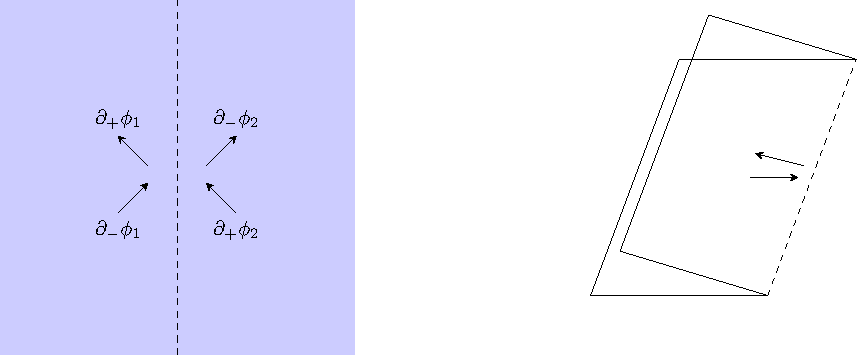
\includegraphics[width=0.45\textwidth]{fig_folding_pic.pdf}
\caption{Folding picture for the penetrable interface. Left panel: World line of the penetrable interface. $\partial_\pm\phi^{1,2}$ denote the left and right going modes in their respective domains. Right panel: Folding operation that sends $\phi^2(x)$ to $\phi^2(-x)$. The dashline represents the \emph{im}penetrable boundary for the resulting tensor theory. The arrow represents the incoming and outgoing particles scattered by the interface.}
\label{fig:folding_pic}
\end{figure}

We now work in the folding picture as shown in Fig.~\ref{fig:folding_pic}. The boundary at $x=0$ becomes impenetrable for the folded system, and the resulting tensor theory admits a conformal invariant boundary state. The folding sends $\phi^2(x)$ to $\phi^2(-x)$ and hence the gluing condition becomes
\begin{equation}
\begin{aligned}
\partial_t(\sin\theta\phi^1-\cos\theta\phi^2)=0, \quad
\partial_x(\cos\theta\phi^1+\sin\theta\phi^2)=0, 
\end{aligned}
\end{equation}
for the case $M = M_1(\theta)$. 

If we quantize the boson theory on the interface line $x = 0$, these gluing conditions become an identity for the boson creation and annihilation operators. We shall interpret these identities to be valid only when acting on the boundary states. The mode expansion of free boson at $x = 0$\cite{di_francesco_conformal_1997} is
\begin{equation}
\label{eq:di_mode_expansion}
\begin{aligned}
\phi(z, \bar{z} ) &= \phi_0 - \frac{i}{4\pi g } \pi_0 \ln z \bar{z} \\
 \quad&+ \frac{i}{\sqrt{4\pi g} } \sum_{n \ne 0 } \frac{1}{n} \left(a_n z^{-n} + \bar{a}_{n} \bar{z}^{-n}   \right),
\end{aligned}
\end{equation}
where we take the following choice of the holomorphic and anti-holomorphic coordinates
\begin{equation}
z= e^{ \frac{2\pi i(x - t)}{T} }, \quad \bar{z} = e^{ \frac{2\pi i( x + t  )}{T} },
\end{equation}
with $T$ being the time period. We end up with a set of operator identities for each mode
\begin{equation}
\begin{aligned}
\label{eq:rotation_a_basis}
\sin  \theta a^1_n - \cos \theta a^2_n  &= + \left( \sin  \theta \bar{a}^1_{-n} - \cos \theta \bar{a}^2_{-n} \right),\\
\cos  \theta a^1_n + \sin \theta a^2_n  &= - \left( \cos  \theta \bar{a}^1_{-n} + \sin \theta \bar{a}^2_{-n} \right), 
\end{aligned}
\end{equation}
which is valid for the following boundary state
\begin{equation}
\label{eq:bd_state}
\begin{aligned}
| B \rangle 
& =  \exp\Big\{ -\sum_{n > 0 } \frac{1}{n}
\begin{pmatrix}
a_{-n}^1\\
a_{-n}^2\\                              
\end{pmatrix}
S_1( \theta )
\begin{pmatrix}
\bar{a}_{-n}^1  \bar{a}_{-n}^2
\end{pmatrix} \Big\} |0\rangle,
\end{aligned}
\end{equation}
where $S_1(\theta) $ is precisely the scattering matrix in Eq.~\eqref{eq:def_S}. The calculation for the case $M=M_2(\theta)$ is completely analogous and we just have a replacement of $S_1( \theta ) $ by $S_2( \theta )$ in Eq.~\eqref{eq:def_S}. 

The boundary state expression in Eq.~\eqref{eq:bd_state} will be used extensively in the fidelity and Loschmidt echo calculation in Sec.~\ref{sec:analytic_numerics}. 

So far the derivation is only for the non-compact bosons, where the interface is determined by the ``gluing conditions''. For the case of connecting compact bosons of different radii, we will need to generalize the relation in Eq.~\eqref{eq:rotation_a_basis} to the winding mode operator $a_0$. Because the winding modes live on a compactification lattice, not all $\theta$ can satisfy Eq.~\eqref{eq:rotation_a_basis} for $a_0$. App.~\ref{app:compact_diff_boson} reviews the derivation about how the winding modes constrain the choice of $\theta$. For example, the $S_1(\theta)$ interface should satisfy
\begin{equation}
\lambda = \tan \theta = \frac{n_2 R_1}{n_1 R_2}
\end{equation}
for coprime integer $n_1$ and $n_2$ and compactification radii $R_1$ and $R_2$ for the bosons on the two sides. This also suggests that connecting two different CFTs will generate an interface whose transmission coefficient are determined by the universal parameters of the CFTs on both sides. 

The winding modes however do not contribute to the fidelity and echo exponent to the leading order, as shown in App.~\ref{app:compact_diff_boson}. So the derivations with the non-compact boson boundary state in Eq.~\eqref{eq:bd_state} holds true for the compact bosons.

%%% Local Variables:
%%% TeX-master: "bCFT_paper"
%%% TeX-PDF-mode: t
%%% End:
